\documentclass[11pt,preprint, authoryear]{elsarticle}

\usepackage{lmodern}
%%%% My spacing
\usepackage{setspace}
\setstretch{1.2}
\DeclareMathSizes{12}{14}{10}{10}

% Wrap around which gives all figures included the [H] command, or places it "here". This can be tedious to code in Rmarkdown.
\usepackage{float}
\let\origfigure\figure
\let\endorigfigure\endfigure
\renewenvironment{figure}[1][2] {
    \expandafter\origfigure\expandafter[H]
} {
    \endorigfigure
}

\let\origtable\table
\let\endorigtable\endtable
\renewenvironment{table}[1][2] {
    \expandafter\origtable\expandafter[H]
} {
    \endorigtable
}


\usepackage{ifxetex,ifluatex}
\usepackage{fixltx2e} % provides \textsubscript
\ifnum 0\ifxetex 1\fi\ifluatex 1\fi=0 % if pdftex
  \usepackage[T1]{fontenc}
  \usepackage[utf8]{inputenc}
\else % if luatex or xelatex
  \ifxetex
    \usepackage{mathspec}
    \usepackage{xltxtra,xunicode}
  \else
    \usepackage{fontspec}
  \fi
  \defaultfontfeatures{Mapping=tex-text,Scale=MatchLowercase}
  \newcommand{\euro}{€}
\fi

\usepackage{amssymb, amsmath, amsthm, amsfonts}

\def\bibsection{\section*{References}} %%% Make "References" appear before bibliography


\usepackage[round]{natbib}

\usepackage{longtable}
\usepackage[margin=2.3cm,bottom=2cm,top=2.5cm, includefoot]{geometry}
\usepackage{fancyhdr}
\usepackage[bottom, hang, flushmargin]{footmisc}
\usepackage{graphicx}
\numberwithin{equation}{section}
\numberwithin{figure}{section}
\numberwithin{table}{section}
\setlength{\parindent}{0cm}
\setlength{\parskip}{1.3ex plus 0.5ex minus 0.3ex}
\usepackage{textcomp}
\renewcommand{\headrulewidth}{0.2pt}
\renewcommand{\footrulewidth}{0.3pt}

\usepackage{array}
\newcolumntype{x}[1]{>{\centering\arraybackslash\hspace{0pt}}p{#1}}

%%%%  Remove the "preprint submitted to" part. Don't worry about this either, it just looks better without it:
\makeatletter
\def\ps@pprintTitle{%
  \let\@oddhead\@empty
  \let\@evenhead\@empty
  \let\@oddfoot\@empty
  \let\@evenfoot\@oddfoot
}
\makeatother

 \def\tightlist{} % This allows for subbullets!

\usepackage{hyperref}
\hypersetup{breaklinks=true,
            bookmarks=true,
            colorlinks=true,
            citecolor=blue,
            urlcolor=blue,
            linkcolor=blue,
            pdfborder={0 0 0}}


% The following packages allow huxtable to work:
\usepackage{siunitx}
\usepackage{multirow}
\usepackage{hhline}
\usepackage{calc}
\usepackage{tabularx}
\usepackage{booktabs}
\usepackage{caption}


\newenvironment{columns}[1][]{}{}

\newenvironment{column}[1]{\begin{minipage}{#1}\ignorespaces}{%
\end{minipage}
\ifhmode\unskip\fi
\aftergroup\useignorespacesandallpars}

\def\useignorespacesandallpars#1\ignorespaces\fi{%
#1\fi\ignorespacesandallpars}

\makeatletter
\def\ignorespacesandallpars{%
  \@ifnextchar\par
    {\expandafter\ignorespacesandallpars\@gobble}%
    {}%
}
\makeatother

\newenvironment{CSLReferences}[2]{%
}

\urlstyle{same}  % don't use monospace font for urls
\setlength{\parindent}{0pt}
\setlength{\parskip}{6pt plus 2pt minus 1pt}
\setlength{\emergencystretch}{3em}  % prevent overfull lines
\setcounter{secnumdepth}{5}

%%% Use protect on footnotes to avoid problems with footnotes in titles
\let\rmarkdownfootnote\footnote%
\def\footnote{\protect\rmarkdownfootnote}
\IfFileExists{upquote.sty}{\usepackage{upquote}}{}

%%% Include extra packages specified by user
\usepackage{booktabs}
\usepackage{longtable}
\usepackage{array}
\usepackage{multirow}
\usepackage{wrapfig}
\usepackage{float}
\usepackage{colortbl}
\usepackage{pdflscape}
\usepackage{tabu}
\usepackage{threeparttable}
\usepackage{threeparttablex}
\usepackage[normalem]{ulem}
\usepackage{makecell}
\usepackage{xcolor}

%%% Hard setting column skips for reports - this ensures greater consistency and control over the length settings in the document.
%% page layout
%% paragraphs
\setlength{\baselineskip}{12pt plus 0pt minus 0pt}
\setlength{\parskip}{12pt plus 0pt minus 0pt}
\setlength{\parindent}{0pt plus 0pt minus 0pt}
%% floats
\setlength{\floatsep}{12pt plus 0 pt minus 0pt}
\setlength{\textfloatsep}{20pt plus 0pt minus 0pt}
\setlength{\intextsep}{14pt plus 0pt minus 0pt}
\setlength{\dbltextfloatsep}{20pt plus 0pt minus 0pt}
\setlength{\dblfloatsep}{14pt plus 0pt minus 0pt}
%% maths
\setlength{\abovedisplayskip}{12pt plus 0pt minus 0pt}
\setlength{\belowdisplayskip}{12pt plus 0pt minus 0pt}
%% lists
\setlength{\topsep}{10pt plus 0pt minus 0pt}
\setlength{\partopsep}{3pt plus 0pt minus 0pt}
\setlength{\itemsep}{5pt plus 0pt minus 0pt}
\setlength{\labelsep}{8mm plus 0mm minus 0mm}
\setlength{\parsep}{\the\parskip}
\setlength{\listparindent}{\the\parindent}
%% verbatim
\setlength{\fboxsep}{5pt plus 0pt minus 0pt}



\begin{document}



\begin{frontmatter}  %

\title{Navigating the Stock Market: A Guide to Smart Investing}

% Set to FALSE if wanting to remove title (for submission)




\author[Add1]{Gabriel Rambanapasi}
\ead{rambanapasi44@gmail.com}





\address[Add1]{Stellenbosch University, Stellenbosch, South Africa}

\cortext[cor]{Corresponding author: Gabriel Rambanapasi}

\begin{abstract}
\small{
This paper investigates dividends return predictive signals, focusing on
Dividend Yield (DY) and Dividend Growth (DG) signals, w
}
\end{abstract}

\vspace{1cm}


\begin{keyword}
\footnotesize{
K-Means\sep Clustering \sep Price Momentun \sep Volatility
\sep Diversification \\
\vspace{0.3cm}
}
\end{keyword}



\vspace{0.5cm}

\end{frontmatter}

\setcounter{footnote}{0}



%________________________
% Header and Footers
%%%%%%%%%%%%%%%%%%%%%%%%%%%%%%%%%
\pagestyle{fancy}
\chead{}
\rhead{}
\lfoot{}
\rfoot{\footnotesize Page \thepage}
\lhead{}
%\rfoot{\footnotesize Page \thepage } % "e.g. Page 2"
\cfoot{}

%\setlength\headheight{30pt}
%%%%%%%%%%%%%%%%%%%%%%%%%%%%%%%%%
%________________________

\headsep 35pt % So that header does not go over title




\hypertarget{introduction}{%
\section{Introduction}\label{introduction}}

Consider the prevailing market consensus that anticipates a specific
direction for market conditions. For instance, in the current interest
rate environment, the majority of practitioners believe that in 2024,
the Federal Reserve will initiate interest rate cuts. This is expected
to trigger a chain reaction in valuations across capital markets,
affecting sectors and industries disproportionately. For portfolio
managers, this underscores the importance of carefully scrutinizing
different parts of the stock market to pinpoint companies that can
enhance the risk/return profile of a portfolio. To identify potential
out performers, we set out to use a combination of clustering using
unsupervised machine learning in K-Means Cluserting and factor analysis
which are price momentum and volatility. Essentially, we reduce the
dimensions of our sample data, making it less challenging to uncover
latent relationships in asset performance over various time periods.

\begin{itemize}
\item
  mention the different time periods that were tested, so when it works
  and why it works. How it works needs a dive into the constituents
  themselves.
\item
\end{itemize}

Initially, we assess performance by employing a simple look-back period
to observe performance and risk over 3, 6, and 12 months. It becomes
evident that, on average, factor portfolios perform well over short
investment horizons. However, they exhibit significant risk levels
compared to a market index. Subsequently, we conduct a rolling backtest
to evaluate the robustness of the portfolios formed through our factor
filter. Our findings suggest that, despite their elevated levels of risk
attributed to the low number of stocks in each portfolio, risk-adjusted
performance, as measured by the Sharpe Ratio, consistently outperforms.
However, it is crucial to note that this strategy is effective over
shorter investment horizons. As the investment horizon extends, the
adverse effects of poor diversification become apparent.

\hypertarget{clustering-and-appliactions-to-asset-management}{%
\section{Clustering and Appliactions to Asset
Management}\label{clustering-and-appliactions-to-asset-management}}

Unsupervised machine learning is a type of machine learning that
searches for patterns in datasets with no pre-existing labels and a
minimum of human intervention. One way in which unsupervised learning
can be applied in data science and other quantitive disciplines is
through clustering algorithms. Clustering is the process of grouping
objects based on similar characteristics. The algorithms designed to
cluster, achieve this function by connecting observation through
distances, density of data points, graphs, or various statistical
distributions. For a cluster to have meaning an algorithm has to
maximize intra-cluster similarity and minimize inter-cluster similarity,
such that each cluster contains information that's as dissimilar to
other
clusters(\protect\hyperlink{ref-kassambara2017practical}{Kassambara,
2017}). There exists various forms of cluster algorithms, each that
addresses a broader task of analysis. The algorithms can be divided into
two main types being partitioning clustering and hierarchical
clustering. The major difference between the divisions of clustering is
the partition clustering aims to specify a predetermined number of
clusters whilst does not
(\protect\hyperlink{ref-kassambara2017practical}{Kassambara, 2017}).
Within partition clustering, for data with a small set of variables,
K-means clustering and partitioning around medoids (PAM) are the most
frequently used due to their fast compuation and simplicity. With
K-means, each cluster is represented by the center or means of the data
points belonging to the entire dataset. This makes the algorithm
sensitive to outliers. However with PAM, each cluster is represented by
one of the objects in the cluster. The other partition clustering
algorithm used for datasets with a large number of variables is
Clustering Large Applications (CLARA).

In asset management, key to funds generating superior risk adjusted
returns is efficient portfolio diversification, thus presenting a great
application for partition clustering. Stocks would be separated into
groups through a clustering algorithm to maximize similarity within
groups and minimizes similarity between groups. Thus allowing managers
to select handpick stock to construct a diversified portfolio. Marvin
(\protect\hyperlink{ref-marvin2015creating}{2015}) use fundamental
ratios (turnover and profitability ratios) weighted equally and K-means
clustering to group US technology stocks listed on the NASDAQ and NYSE.
A diversified portfolio is then constructed based on within cluster
stock performance i.e.~stock selected are those that possess the highest
Sharpe ratio. Results over a period of 15 years that included the dot
com bubble and the global financial crises showed that cluster
portfolios exhibited more volatility than the benchmark (S\&P 500),
however returns to investors were above the benchmark at multiples
ranging from 3.5 to 5.7 times when earnings are reinvested into the
cluster portfolios. Bin (\protect\hyperlink{ref-bin2020k}{2020}) uses a
similar approach to Marvin
(\protect\hyperlink{ref-marvin2015creating}{2015}), however employing a
combination of market ratios and fundamental ratios (price to earnings
ratio, return on assets ratio and asset turnover ratio ). From this
study, compared to the S\&P 500, portfolios constructed using market
ratios under performed those that used fundamental ratios. \newpage

\hypertarget{data-and-methodology}{%
\section{Data and Methodology}\label{data-and-methodology}}

This section describes how we obtain the data set used in the study,
details the clustering process and validating metrics employed, to
obtain the results in \ref{Results}. For the methodology results, see
Appendix

\hypertarget{obtaining-and-prepariing-the-dataset}{%
\subsection{Obtaining and prepariing the
dataset}\label{obtaining-and-prepariing-the-dataset}}

The data employed in this paper is based on the constituent list of the
Johannesburg All Share Index (ALSI) from January 1, 2000 to January 15
2024, which contains the list of the 164 companies with the highest
market value and liquidity. The historical price and volume data is
retrieved from Yahoo Finance and fundamental data from Bloomberg. From
historical price data obtained from Yahoo Finance, we filter stock that
have trading volume that exceed 1 000 000 shares traded per year and
exclude stock that have less than 90 percent of observations in the
historical price dataset.

To avoid large oscillations in the data, we transformed the price series
to include end of month data points thus returns calculations are based
on from the monthly data. Monthly historical prices are transformed
using simple returns and we assume that embedded in the price action are
cooperate events such as stock splits or consolidations of the shares.
Therefore there is no need to make additional transformations on the
return series to reflect corporate actions.

The measures of similarity used in this study are volatility and price
momentum. To cluster stock based on the two measures, we apply a
percentile ranking criterion on stock scores during a time period. For
price momentum, describes the causality between relatively strong
performance and high future return and vice-versa. Ranking highly
implies that strong performers and thus higher returns than weak
performers. This study defines cross sectional momentum as the trailing
6 month cumulative return Jegadeesh \& Titman
(\protect\hyperlink{ref-jegadeesh1993returns}{1993}). For volatility,
using a 12 month lock back period compute the standard deviation. The
results of the ranking are shown in Table \ref{tab1}

\hypertarget{stocks-clustering}{%
\subsection{Stocks clustering}\label{stocks-clustering}}

\hypertarget{lloyds-algorithm}{%
\subsubsection{Lloyd's algorithm}\label{lloyds-algorithm}}

We employ the K-means that partitions \(n\) observations into \(k\)
clusters. The goal is to minimize the within cluster sum of squares or
analytically,
\(\underset{s}{\arg \min } \sum_{i=1}^k \sum_{x \in S_i}\left\|x-\mu_i\right\|^2\)
where \(x\) are the observations, \(S=S_1, S_2, \ldots, S_k\) are the
sets of observations, and \(\mu_i\) is the mean of the points in
\(S_i\). To arrive at the optimum number of clusters, we utilize the
most popular algorithm called the Lloyd's algorithm that is closely
followed by Marvin (\protect\hyperlink{ref-marvin2015creating}{2015}),
Bin (\protect\hyperlink{ref-bin2020k}{2020}) \& Xu, Xu \& Wunsch
(\protect\hyperlink{ref-xu2010clustering}{2010}).

Analytically, given a set of points
\(\left\{x_1, \cdots x_n\right\}\left(x_i \in \mathbb{R}^m\right)\),
Initialize the K clusters with \(\left\{C_1, \cdots C_K\right\}\) with
centers.
\(\left\{m_1, m_2, \cdots m_K\right\}\left(m_i \in \mathbb{R}^m\right)\).
The centers are picked using the silhouette method discussed in
\ref{sil} For all points \(x_i(i \in\{1, \cdots n\})\), find the center
that closest based on a euclidean distance \(d\). Following this, assign
\(x_i\) to the cluster corresponding to the closest centre. Then
\(x_i \in C_j\) if
\(d\left(x_i, m_j\right) \leq d\left(x_i, m_l\right) \quad(\forall l \in\{1, \cdots K\})(j \neq l)(\forall i \in\{1, \cdots n\})\).
Recalculate the center for each cluster \(C_l(l \in\{1, \cdots K\})\).
The new cluster centers are the mean of the points in the same cluster.

\(m_l=\frac{1}{\left|C_l\right|} \sum_{x_p \in C_l} x_p \quad(\forall l \in\{1, \cdots K\})\).

Repeat processes two and three until no cluster has any change in point
assignment.

\hypertarget{silhoutte-index}{%
\subsection{\texorpdfstring{Silhoutte index
\label{sil}}{Silhoutte index }}\label{silhoutte-index}}

To evaluate the goodness of fit of partitioning using K means clustering
the silhoutte index is used
(\protect\hyperlink{ref-rousseeuw1987silhouettes}{Rousseeuw, 1987}).
Given \(n\) data points \(\left\{x_1, \cdots x_n\right\}\), a
partitioning result of \(K\) cluster \(\left\{C_1, \cdots C_K\right\}\)
and distance metric \(d\), for each \(x_i\) in cluster \(C_l\), define

\(a\left(x_i\right)=\frac{1}{\left|C_l\right|-1} \sum_{\forall x_j \in C_l, i \neq j} d\left(x_i, x_j\right)\)

\(a(x_i)\) is the mean dissimilarity between \(x_i\) to all other points
within the same cluster.For each point \(x_i\) in cluster \(C_l\),
define

\(b\left(x_i\right)=\min _{\forall p \in\{1, \cdots K\}, p \neq l} \frac{1}{\left|C_p\right|} \sum d\left(x_i, x_j\right.)\)

\(b(x_i)\) is the minimum dissimilarity between \(x_i\) and all points
in some \(C_p\) which does not contain \(x_i\). For each point \(x_i\)
in cluster \(C_l\), their silhouette index is defined as

\(s\left(x_i\right)= \begin{cases}1-\frac{a\left(x_i\right)}{b\left(x_i\right)} & \text { if } a\left(x_i\right)<b\left(x_i\right) \\ 0 & \text { if } a\left(x_i\right)=b\left(x_i\right) \\ \frac{b\left(x_i\right)}{a\left(x_i\right)}-1 & \text { if } a\left(x_i\right)>b\left(x_i\right)\end{cases}\)

where \(s(x_i)\) ranges between \([-1, 1]\). For \(s(x_i)\) that
approaches 1, it means that \(a(x_i)\) needs to be significantly smaller
than \(b(x_i)\), implying that within-cluster mean dissimilarity is much
less than the smallest between-cluster mean dissimilarity, and thus the
model does a good job clustering similar points together.

For the \(s(x_i)\) that approaches 0, \(a(x_i)\) needs to be
significantly greater than \(b(x_i)\), implying that within-cluster mean
dissimilarity is much greater than the smallest between- cluster mean
dissimilarity, and thus the model does a poor job clustering similar
points together.

For this study, we choose \(K\) with the highest silhoutte index/value

\hypertarget{portfolio-backtest}{%
\subsection{Portfolio Backtest}\label{portfolio-backtest}}

The out-of-sample performance of cluster portfolios is compared to the
benchmark, the JSE All Share Index. To manage risk exposure to a single
asset or industry, we use a cap on each asset's allocation. Thus use a
single company methodology similar to Standard \& Poor Capping
Methodology \footnote{see S\&P (\protect\hyperlink{ref-sp}{2023}) for a
  breakdown of the process used to cap an index}. In a single company
capping methodology, no company in an index (cluster in our case) is
allowed to breach a certain pre-determined weight as of each rebalancing
period \footnote{The maximum set for each stock in each cluster is its
  equal weight for that cluster i.e if there were 10 stock in cluster 1,
  the maximum weight would be 10\%}. Theoretically, this should preserve
the within cluster diversification benefits and allow the portfolio
value to either increase or decrease depending on stock performance
during the quarter. We rebalance the portfolios once every three months,
similar to the frequency of rebalancing conducted by the JSE on the
JSE/FTSE indices, that is, re balance on the last daty of March, June,
September and December.

\newpage

\hypertarget{results}{%
\section{\texorpdfstring{Results
\label{Results}}{Results }}\label{results}}

This section will present and analyze the clustering results of the
K-means algorithms. All clusters formed and individual stock risk and
return characteristics are examined. I constrcuted bespoked equally
weighted portfolios then examine their performance against a benchmark.
For illustrations and graphs of the clustering results, see Appendix 1.
A description of the constructed portfolios can be found in Appendix 2
and 3

\hypertarget{clustering-results-of-stock-price-movement-dataset}{%
\subsection{Clustering results of stock price movement
dataset}\label{clustering-results-of-stock-price-movement-dataset}}

For each of the K values, the K-means algorithm is ran 1000 times, and
the average silhouette value for the clustering results is recorded. The
result is shown in Figure 1 in Appendix 1. As is apparent in the gure, K
= 4 yields the optimal silhouette value and K = 6 yields a local optima.
Although a natural choice is K = 11, as S\&P Global divides all
companies into 11 major sectors, this is not optimal since K = 11 has a
relatively small average silhouette value.

\hypertarget{clustering-result-of-k-6}{%
\subsection{Clustering Result of K = 6}\label{clustering-result-of-k-6}}

\hypertarget{cluserting-result-of-k-9}{%
\subsection{Cluserting Result of K = 9}\label{cluserting-result-of-k-9}}

\newpage

\hypertarget{references}{%
\section{References}\label{references}}

\hypertarget{refs}{}
\begin{CSLReferences}{1}{0}
\leavevmode\vadjust pre{\hypertarget{ref-asness2011momentum}{}}%
Asness, C. 2011. Momentum in japan: The exception that proves the rule.
\emph{The Journal of Portfolio Management}. 37(4):67--75.

\leavevmode\vadjust pre{\hypertarget{ref-bin2020k}{}}%
Bin, S. 2020. K-means stock clustering analysis based on historical
price movements and financial ratios.

\leavevmode\vadjust pre{\hypertarget{ref-jegadeesh1993returns}{}}%
Jegadeesh, N. \& Titman, S. 1993. Returns to buying winners and selling
losers: Implications for stock market efficiency. \emph{The Journal of
finance}. 48(1):65--91.

\leavevmode\vadjust pre{\hypertarget{ref-kassambara2017practical}{}}%
Kassambara, A. 2017. \emph{Practical guide to cluster analysis in r:
Unsupervised machine learning}. Vol. 1. Sthda.

\leavevmode\vadjust pre{\hypertarget{ref-marvin2015creating}{}}%
Marvin, K. 2015. Creating diversified portfolios using cluster analysis.
\emph{Princeton University}.

\leavevmode\vadjust pre{\hypertarget{ref-rousseeuw1987silhouettes}{}}%
Rousseeuw, P.J. 1987. Silhouettes: A graphical aid to the interpretation
and validation of cluster analysis. \emph{Journal of computational and
applied mathematics}. 20:53--65.

\leavevmode\vadjust pre{\hypertarget{ref-sp}{}}%
S\&P. 2023. \emph{Index mathematics methodology}.

\leavevmode\vadjust pre{\hypertarget{ref-xu2010clustering}{}}%
Xu, R., Xu, J. \& Wunsch, D.C. 2010. Clustering with differential
evolution particle swarm optimization. In IEEE \emph{IEEE congress on
evolutionary computation}. 1--8.

\end{CSLReferences}

\newpage

\hypertarget{appendix}{%
\section{Appendix}\label{appendix}}

\hypertarget{appendix-a}{%
\subsection{Appendix A}\label{appendix-a}}

\begingroup\fontsize{12pt}{13pt}\selectfont
\begin{longtable}{lrr}
  \toprule
Ticker & Volatility  Rank & Price Momentum Rank \\ 
  \hline 
\endhead 
\hline 
{\footnotesize Continued on next page} 
\endfoot 
\endlastfoot 
 \midrule
ABG & 26.67 & 21.67 \\ 
  ANG & 16.67 & 16.67 \\ 
  BIK & 80.00 & 73.33 \\ 
  EQU & 90.00 & 86.67 \\ 
  FFA & 3.33 & 53.33 \\ 
  GFI & 50.00 & 30.00 \\ 
  GLN & 56.67 & 36.67 \\ 
  HAR & 46.67 & 100.00 \\ 
  HMN & 66.67 & 60.00 \\ 
  KAP & 70.00 & 33.33 \\ 
  KBO & 100.00 & 3.33 \\ 
  MCG & 73.33 & 43.33 \\ 
  MRP & 10.00 & 46.67 \\ 
  MTM & 60.00 & 76.67 \\ 
  NPH & 96.67 & 26.67 \\ 
  ORN & 30.00 & 10.00 \\ 
  OUT & 20.00 & 56.67 \\ 
  PAN & 33.33 & 83.33 \\ 
  PIK & 36.67 & 6.67 \\ 
  PPC & 83.33 & 95.00 \\ 
  QLT & 53.33 & 90.00 \\ 
  RMH & 86.67 & 95.00 \\ 
  SAP & 43.33 & 80.00 \\ 
  SBK & 13.33 & 70.00 \\ 
  SOL & 40.00 & 13.33 \\ 
  TCP & 93.33 & 63.33 \\ 
  TFG & 23.33 & 40.00 \\ 
  TRU & 6.67 & 50.00 \\ 
  VKE & 76.67 & 66.67 \\ 
  WHL & 63.33 & 21.67 \\ 
   \bottomrule
\caption{Clustering Similarity Measures\label{tab1}} 
\end{longtable}
\endgroup

\begin{figure}[H]

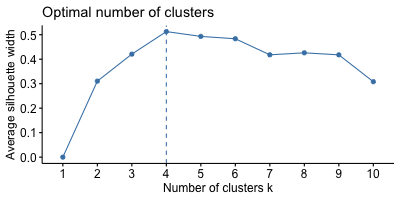
\includegraphics[width=5.56in]{images/silhouette} \hfill{}

\caption{ Silhoutte Indexes for Clusters \label{fig1}}\label{fig:unnamed-chunk-2}
\end{figure}

\begin{figure}[H]

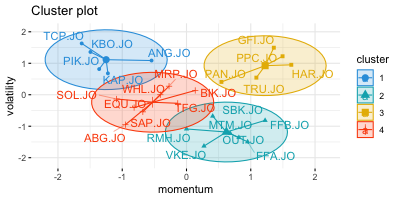
\includegraphics[width=5.56in]{images/clusters_image} \hfill{}

\caption{ Clusters Results from Highest Silhoutte \label{fig2}}\label{fig:unnamed-chunk-3}
\end{figure}

\hypertarget{appendix-b}{%
\subsection{Appendix B}\label{appendix-b}}

\bibliography{Tex/ref}





\end{document}
